%# -*- coding: utf-8-unix -*-
%%==================================================
%% chapter02.tex for SJTU Master Thesis
%% based on CASthesis
%% modified by wei.jianwen@gmail.com
%% Encoding: UTF-8
%%==================================================

\chapter{基于异常数据的入侵检测设计}
\label{chap:data detection}

\section{引言}
\label{sec:intro}

在上一章节中,我们讨论了过程控制系统在远程输入信号采集和传输过程中遭受的数据注入攻击并阐述如何构造较为隐蔽的错误序列注入攻击。事实上大多数控制应用(例如监控和数据采集(SCADA))都需要保证严格的安全性,因为一旦由任何异常故障或恶意攻击引起的错误甚至恶意行为都会导致物理设备甚至整个系统遭受无法逆转的破害。在本章节中,我们主要针对控制系统中控制器接收来自本地和远程输入信号的完整性和安全性设计了基于异常数据的入侵检测机制,并且我们考虑到错误序列注入攻击序列构造特性设计了有效的FSI检测算法。

\section{入侵检测方案概述}
\label{sec:list}

考虑到前一章节中描述的威胁模型,来自远程终端单元(RTU)或PLC的远程传感器的信号数据也面临数据集成攻击,我们将入侵检测机制放在PLC或者RTU可编程控制器与物理设备连接的输入和输出两端。从传感器测量的每个数据或信号都需要经过监测并验证完整性,一旦存在未能通过检测的观测数据机制立即给出报警并定位可能受攻击的传感器位置。具体实现时,与构造攻击采用的模型辨识类似,首先收集PLC控制器与系统物理设备之间传输的信号和内存数据形成输入和输出向量采样数据库,我们辨识出能够高度复现待检测系统的无故障离散事件模型。然后针对异常数据注入攻击的特点,分为两个阶段设计异常数据检测算法。第一阶段将监测的控制器输入信号与模型的预期输出残差对比判断是否数据异常;第二阶段对隐蔽的错误序列注入攻击设计额外FSI检测算法来避免此类型的攻击。最后对检测存在异常的数据分析判断,定位到具体攻击源并给出相应的应对措施。



\section{系统建模和入侵检测设计}
\label{sec:matheq}

\subsubsection {攻击类型}

对于异常数据注入攻击,主要存在两种类型。一类是\textit {蛮力和类故障攻击},例如由Mclaughlin等人提出的拥有控制意识的FDI攻击\parencite{mclaughlinS2014}和由Pang等人设计的伪装假数据攻击\parencite{pang2015}。 然而这类攻击是实现具体的任务和目标是销毁受控系统,但是没有考虑受感染系统本身的安全机制,所以很容易被成熟的故障检测机制检测到\parencite{roth2012,garcia2012}。另一类是\textit {隐蔽和避免故障检测的攻击},这类攻击的典型代表就是我们前一章节构造的错误序列注入攻击。这种类型的攻击要求攻击者熟悉的受感染系统的物理变量与控制器连接配置信息并能够访问传感器,因此它可以避开系统故障检测。

\subsubsection {检测方法}

我们在图\ref {fig28}中创建了一个两阶段检测的流程示意图,用于描述基于前一节提到的两种类型的攻击进行基于异常数据的检测过程。 一方面图\ref {fig28}显示了结合观测到的I$I/O$向量数据库和辨识的离散事件模型,我们首先对a)类攻击\textit {蛮力和类故障攻击}进行残差对比检测。另一方面我们需要验证当前观测的向量值映射到模型中的状态的前一状态是否存在多个后继状态,对应到状态转移图即当前对应的状态只是上一状态的某个分支其,如果是的话我们针对b)类攻击\textit {隐蔽和避免故障检测的攻击}进行特定的FSI检测。最后在经过两个阶段检测之后,我们将检测结果进行分析并定位以获得攻击源的具体位置。

\begin{figure}[!htb]
		\centering
		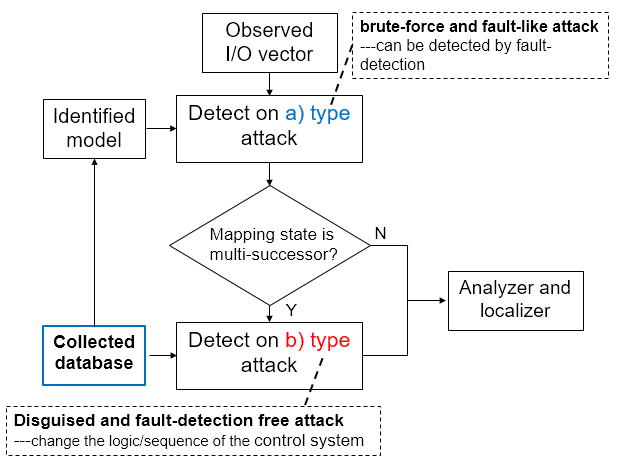
\includegraphics[scale=0.35]{dataD/flow-chart.png}
		\caption{基于异常数据检测的流程示意图}
		\label{fig28}
	\end{figure}

考虑到我们的主要检测目标是能够改变控制系统的逻辑或进程的错误序列注入攻击,由于FSI攻击来自辨识的模型的相同输出确保其不会被故障机制直接检测,而且通过选择具有恶意执行逻辑的适当长度的错误序列注入到控制器的输入信号中来破坏系统。算法\ref{algo:abd}显示了基于异常数据的检测过程。第一步是通过类似构造攻击模型辨识过程来获得待检测系统NDAAO模型,然后根据残差计算每个当前观测的$I/O$向量值与模型的预期输出是否一致。如果不一致则认为在当前模型的状态估计集为空即不存在任何可行的下个状态,此时很可能遭受\textit{蛮力和类故障攻击},否则我们需要检查先前状态估计集模$|\hat{X}_{t-1}|$的大小是否大于1,如果是的话可能存在错误序列注入攻击并进行第二阶段FSI攻击的检测。

由上章节中FSI序列的定义式(2-7)中长度为$n$的序列$s$满足的必要条件是$s\notin L_{Obs}^n$,所以我们需要增加记录每一观测向量值并判断从观测周期初始向量到当前观测向量组成的观测序列$\phi$是否存在与原始用来辨识模型的采样序列库中,如果不存在的话则可以判断系统受到FSI攻击。为了使检测更加有效,我们只保留每次检测时序列满足$ \varphi$属于$\gamma'$任意子字符串的$\gamma'$并将$\gamma'$保存于$\varSigma'$,主要目的是删除没有用到的验证序列集并保留有效的序列以验证观测序列$\phi$是否属于采样序列库的子串。 此外介于相邻两个多后继状态之间的序列是唯一的,我们仅仅判断$ \varphi $和$ \gamma $的多后继映射向量(包括当前向量)序列更快地进行验证。 最后判断当前估计状态集$|\hat{X}_{t}|$是否是否等于1,如果不是的话我们把控制系统视为受到\textit {隐蔽和避免故障检测的攻击},否则控制系统将安全地通过检测即没有受到任何攻击。

\begin{algorithm}[h]
		\caption{基于异常数据的检测算法}
		\label{algo:abd}
		\begin{algorithmic}[1]
			\Require %算法的输入参数:Input  
			辨识的NDAAO模型, 新观测的$I/O$向量$\varphi(t)$, 模型的状态估计$|\hat{X}_{t-1}|$, 和用于模型辨识的采样序列库$\varSigma$ \\  
			\Ensure %算法的输出:Output  
			是否通过检测,如果没有的话系统可能受到的攻击类型并给出系统受攻击的路径和传感器位置$locatePair$。 \\
			\If {$|$\^{X}$_{t-1}$$| > 0$}
			\State \^{X}$_{t}$ $\leftarrow \{x\in X|\exists x_{pre}\in$ \^{X}$_{t-1}$$:x\in f(x_{pre}) \wedge IO(\lambda(x_{pre}),\lambda(x))=IO(\lambda(x_{pre}),\varphi(t))\}$
			\If {$|\hat{X}_t|=0$}
			\State $locatePair\leftarrow locatePair((\varphi_{init},...,\varphi(t)),IO(\lambda(x_{pre})\cup IO(\lambda(x_{pre}),\varphi(t)))$
			\State \textbf{return} \textit{蛮力和类故障攻击}
			\EndIf
			\If {$deg(\hat{X}_{t-1})>1$}
			\State $\phi \leftarrow (\varphi_{init},...,\varphi(t))$
			\For {each $\gamma \in \varSigma$}
			\State 保留满足 $\varphi 属于\gamma'$子串的$\gamma'$ 并且 $\varSigma' \leftarrow \gamma'$
			\State $\phi_{ms} \leftarrow$ 保留对应到模型中的多后继向量(包括当前向量)的 $\phi$的序列
			\State $\gamma_{ms} \leftarrow$ 保留对应到模型中的多后继向量(包括当前向量)的 $\gamma$的序列
			\State $\phi\leftarrow \phi_{ms}, \gamma\leftarrow \gamma_{ms}$
			\If {$\phi \notin substring(\gamma)$}
			\State $\hat{X}_t \leftarrow \emptyset$
			\State break
			\EndIf
			\EndFor
			$\varSigma \leftarrow \varSigma'$
			\EndIf
			\Else
			\State $\hat{X}_t \leftarrow \{x\in X|\lambda(x)=\varphi(t)\}$
			\EndIf
			$\hat{X}_{t-1}\leftarrow \hat{X}_t$
			\If {$|\hat{X}_t|=1$}
			\State \textbf{return} \textit{安全通过检测}
			\Else
			\State $locatePair\leftarrow locatePair(\phi,IO(\lambda(x_{pre})\cup
			IO(\lambda(x_{pre}),\varphi(t)))$
			\State \textbf{return} \textit{隐蔽和避免故障检测的攻击}
			\EndIf
		\end{algorithmic}
	\end{algorithm}








\begin {table}[!htb]
\caption {ds1006的技术细节}
\begin{tabular} {|p{4cm}|p{10cm}|} \hline \hline

  参数&规格\\ \hline
  处理器&四核AMD皓龙处理器2.8 GHz,4 x 64 kB L1数据高速缓存,4 x 64 kB L1指令高速缓存,4 x 512 kB L2高速缓存,6 MB L3高速缓存\\ \hline
  定时器&每个内核:3个通用定时器,多处理器系统的同步时基单元(STBU)\\ \hline
  中断控制器&每个内核:一个中断控制器,具有18个不同的中断源,连接的I/O板的中断源可以通过内部Gigalink从每个内核处理。 \\ \hline

  接口&RS232接口,标准UART允许传输速率高达115.2 Kbaud(串行)\\ \hline
  接口(连接到I/O板)&PHS ++总线接口,用于模块化I/O配置的32位I/O总线(第374页),峰值传输速率为20 MB / s,新I/O板,最多64个PHS总线中断。 \\ \hline

  主机接口&一个全尺寸16位ISA插槽,通过8个16位I/O端口(ISA总线)接口\\ \hline

  多处理器系统&构建具有更多DS1006处理器板的多处理器系统,多达20个DS1006处理器板,每个DS1006上通过一个DS911千兆模块最多4条高速链路,可能的电缆长度可达100米\\ \hline

  物理特性&340 x 125 x 15毫米(13.4 x 4.9 x 0.6英寸)(物理尺寸)\\ \hline
  物理特性&0-40°C(32-104°F)(环境温度)\\ \hline
  物理特性&主动冷却(风扇)(冷却)\\ \hline
  物理特性&(电源)ISA总线:+5 V±5%2.0 A(无DS911),+5 V±5%3.0 A(DS911至模块版本2.0),+12 V±5%连接器:+5 V±5%20 A. \\ \hline


  内存&1 GB DDR2-800 SDRAM本地内存,用于应用程序和动态应用程序数据,4 x 128 MB DDR2-267 SDRAM全局内存,用于主机数据交换\\ \hline\hline
\end{tabular}
\end{table}

\section{实验仿真}
\label{sec:insertimage}

\section{本章小结}
\label{sec:insertimage}

